\section{City Utilities, Facilities, and Services}

\subsection{Water and Sanitation}

\noindent Second only to land availability, the provision of clean water and sanitary sewer services is the most important factor that impacts the city's ability to sustain itself and grow. Furthermore, utility services are important sources of city revenue. This is only possible if the customer base is growing and the rates charged to customers cover the cost of providing clean water and sanitation.\\

\noindent The \href{https://bloomfieldnebraska.com/government/}{City of Bloomfield Website} describes these utilities:

\subsubsection*{Water System}
\begin{quote}
    The city water system includes three supply wells with a total production capacity of approximately 1,000 gallons per minute. The average daily demand is 180,000 gallons with a maximum capacity of 1,440,000 per day. The static pressure is 93 pounds and the residual pressure is 86 pounds. The system also includes a single 250,000 elevated storage tank constructed in 1996. Extensive upgrades were undertaken in the water system between 1995 and 1997 resulting in an 8″ water line loop around the city. The quality of water in Bloomfield does not necessitate treatment.
\end{quote}

\subsubsection*{Sewer System}
\begin{quote}
    The wastewater system consists of approximately 6.9 miles of gravity collection mains, a satellite lift station in the east part of the city and a main lift station at the city park pumping all wastewater through a 3,200 foot 6″ force main to a four cell lagoon system. The collection system includes about 1,000 feet of 12″ main, 4,500 feet of 10″ main, 22,000 feet of 8″ main and 4,200 feet of 4″ main. The four cell lagoon is operated as a controlled discharge system and was upgraded within the last 10 years. It meets the state NPDES limits on effluent. Renovations of the main lift station and collection system are being done in 2000, including a new lift station on the west side of the city.
\end{quote}

\pagebreak
\noindent On the whole, Bloomfield residents are more satisfied than dissatisfied with the provision of water and sewer utilities. \textbf{Figure~\ref{fig:scoreWaterSewer}} shows that Bloomfield residents were 18 percent more likely to rate the city water service as "good" or better, and 14 percent more likely to rate the city sewer service as "good" or better.

\begin{figure}[H]
\centering
\begin{framed}
    \caption{Assessment of Water and Sewer Utilities}
    \label{fig:scoreWaterSewer}
    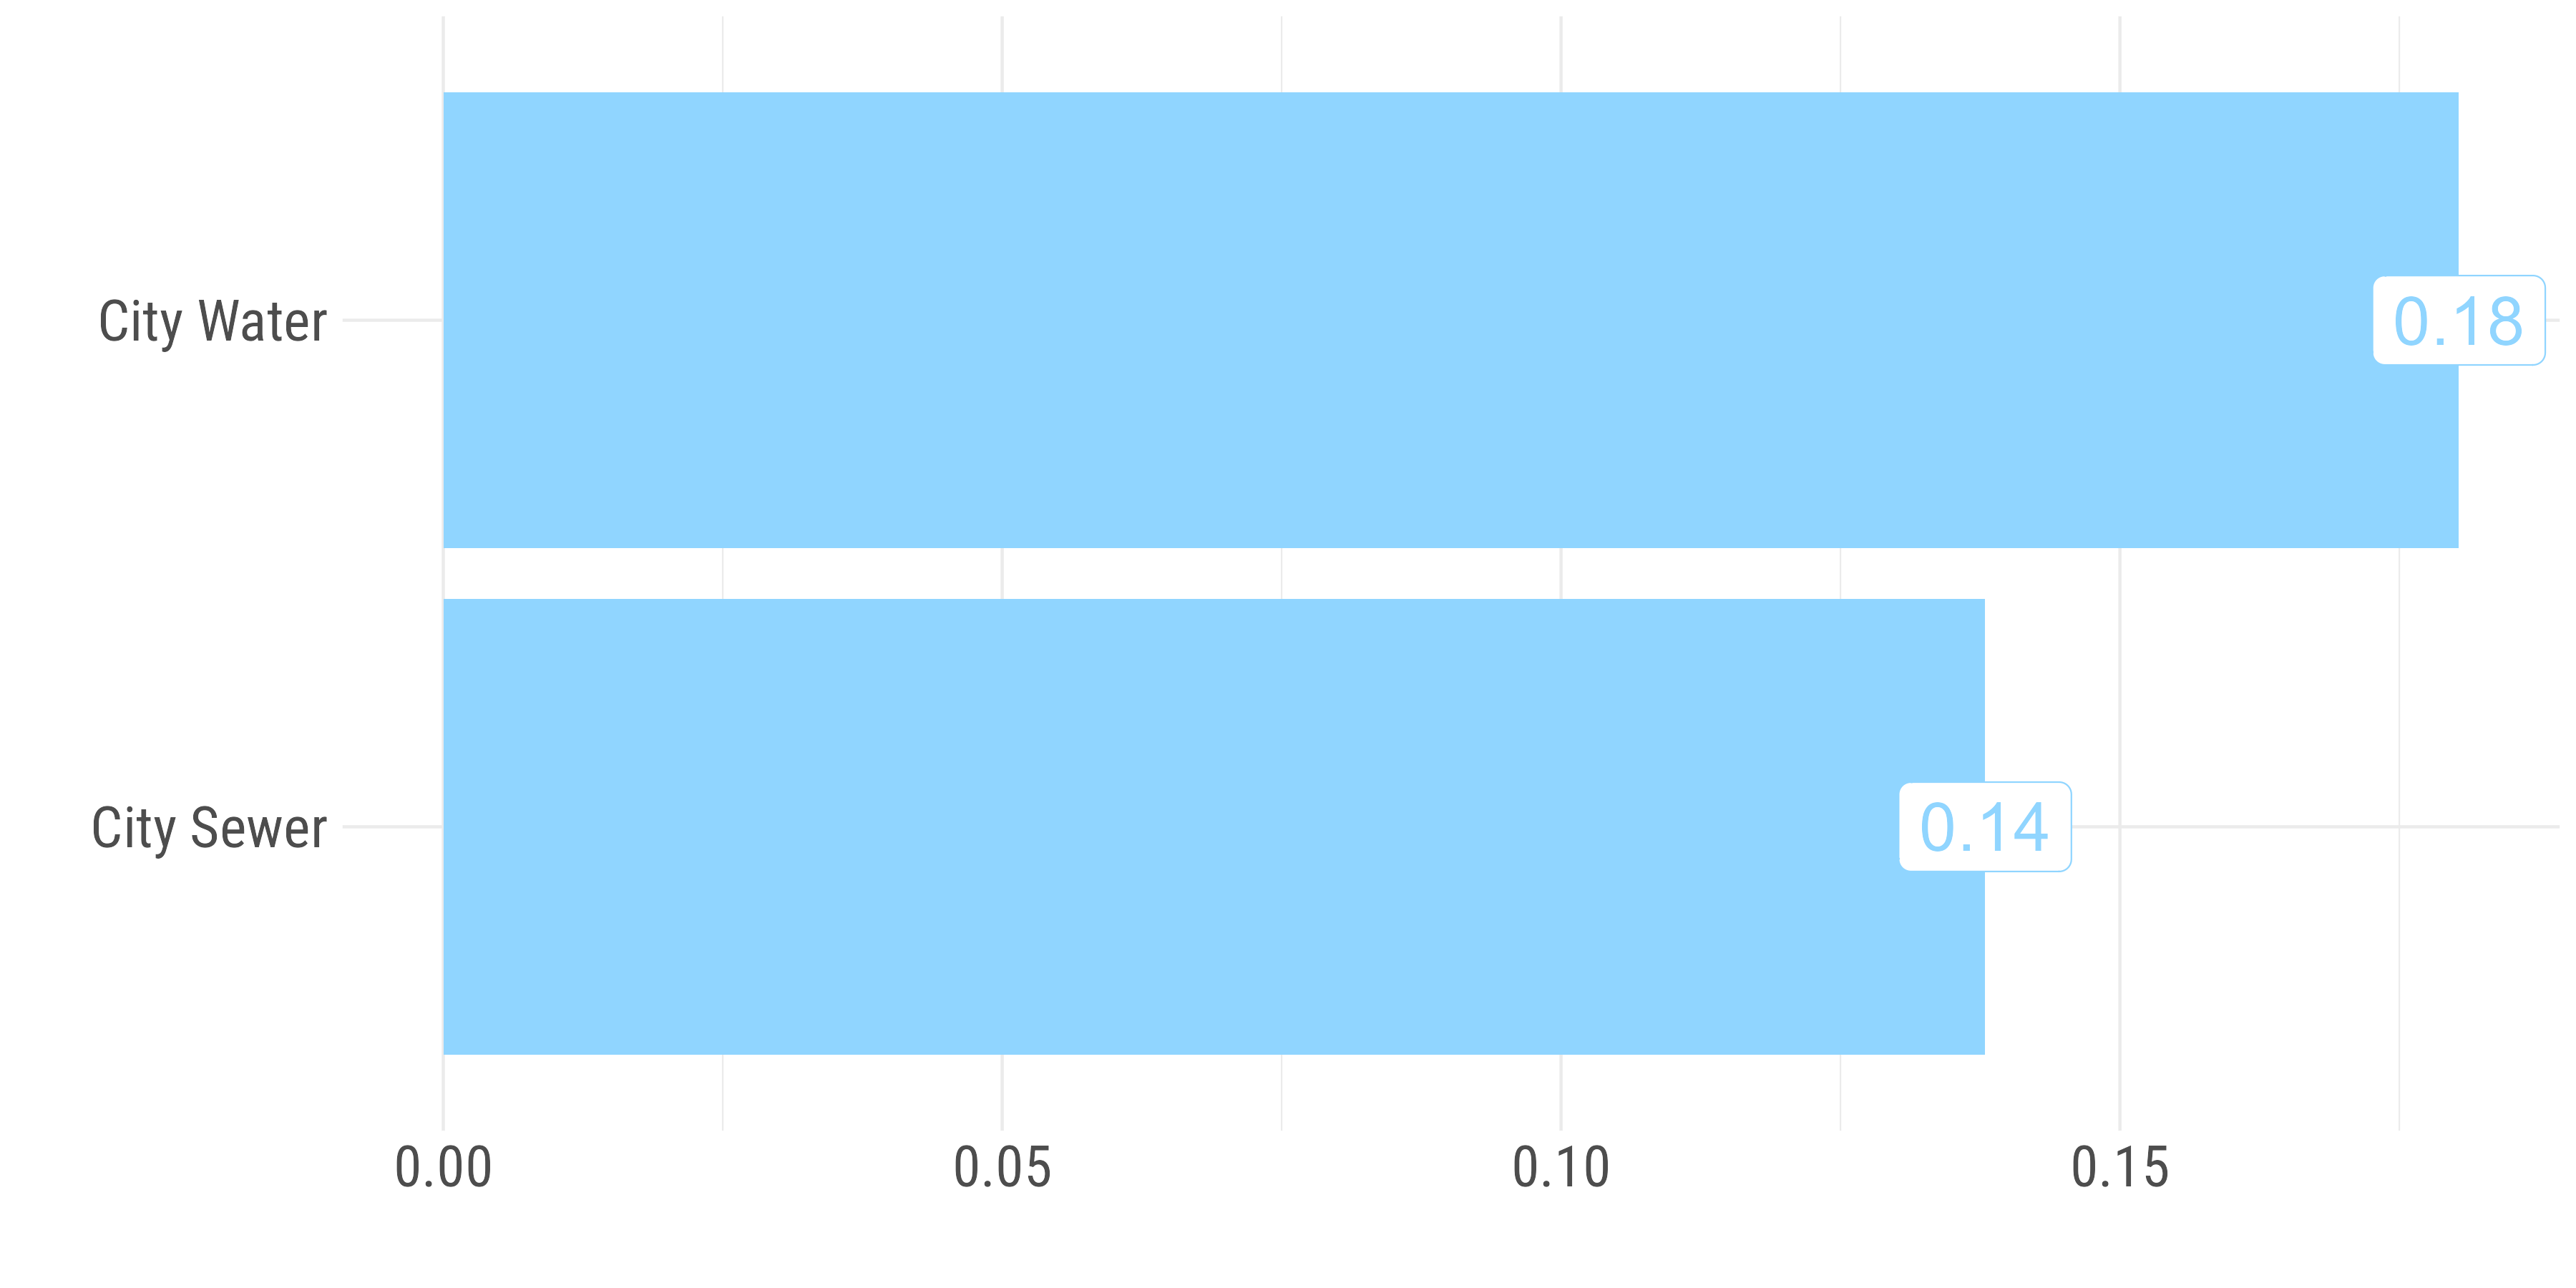
\includegraphics[width = \linewidth]{figures/score_water_sewer.png}
\end{framed}
\end{figure}

\noindent The maps on the following pages detail the location of Bloomfield's water and sewer infrastructure.

\pagebreak
\thispagestyle{empty}
\begin{landscape}
    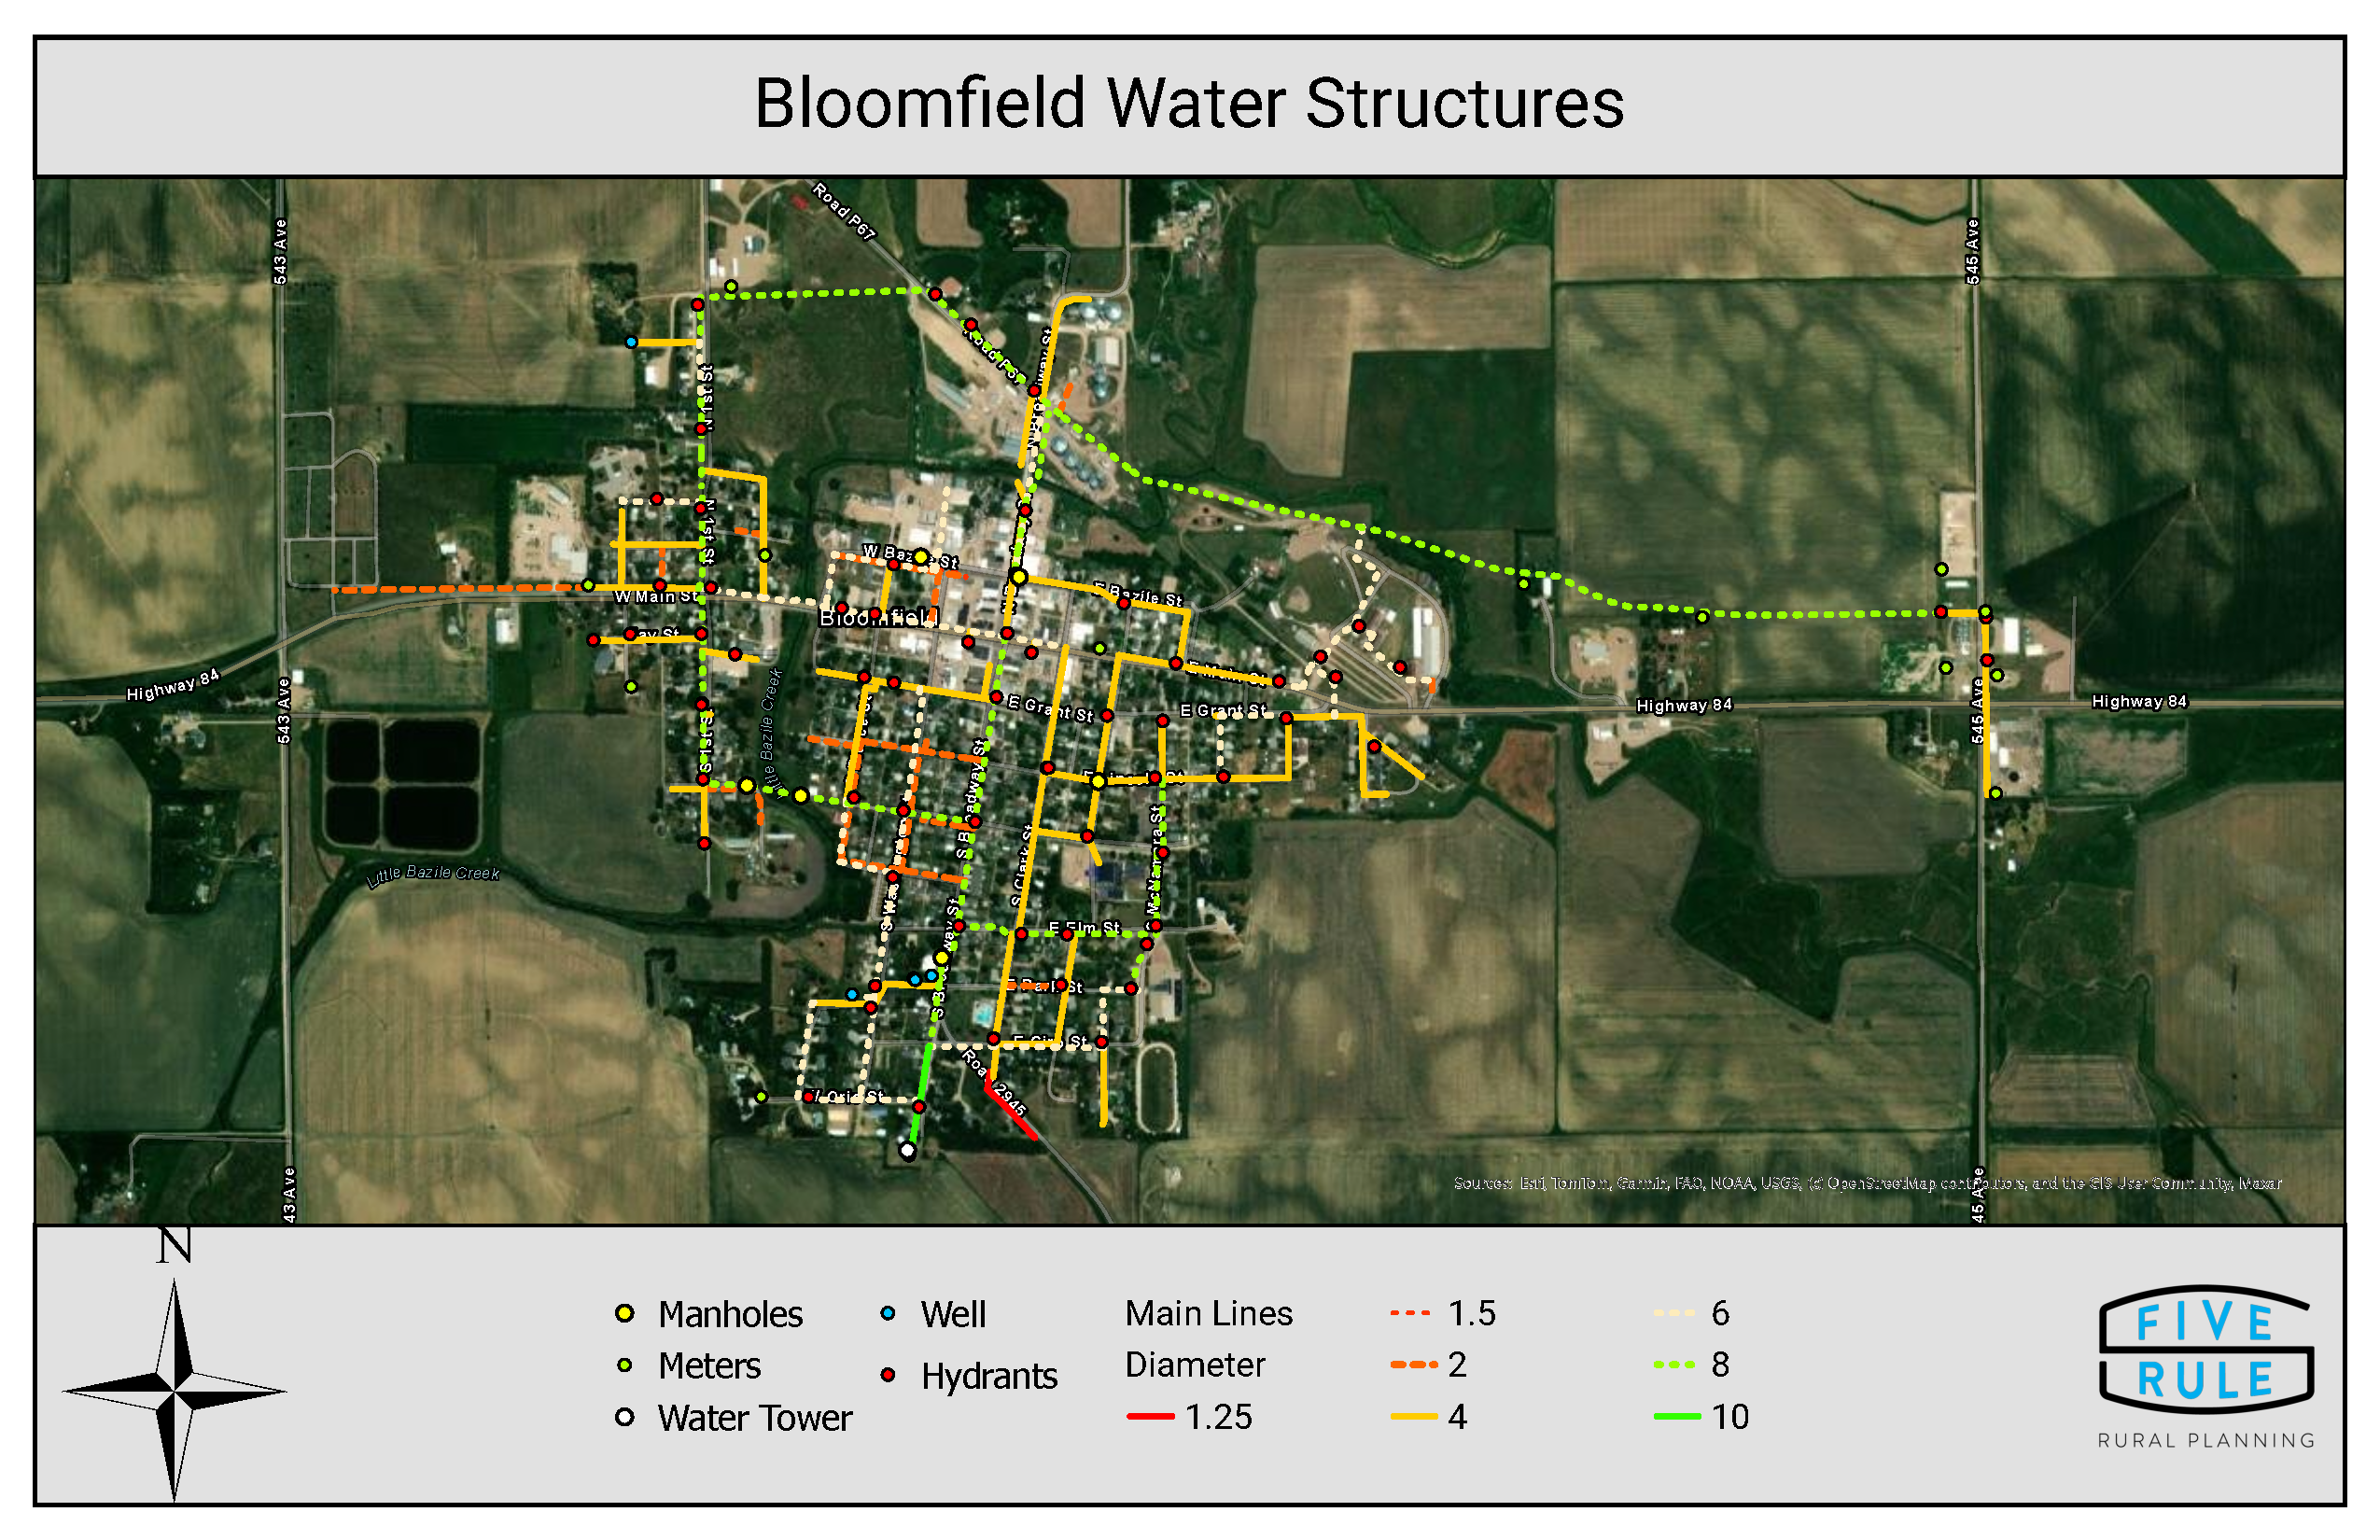
\includepdf[angle = 90]{maps/water_structures.pdf}
\end{landscape}

\pagebreak
\thispagestyle{empty}
\begin{landscape}
    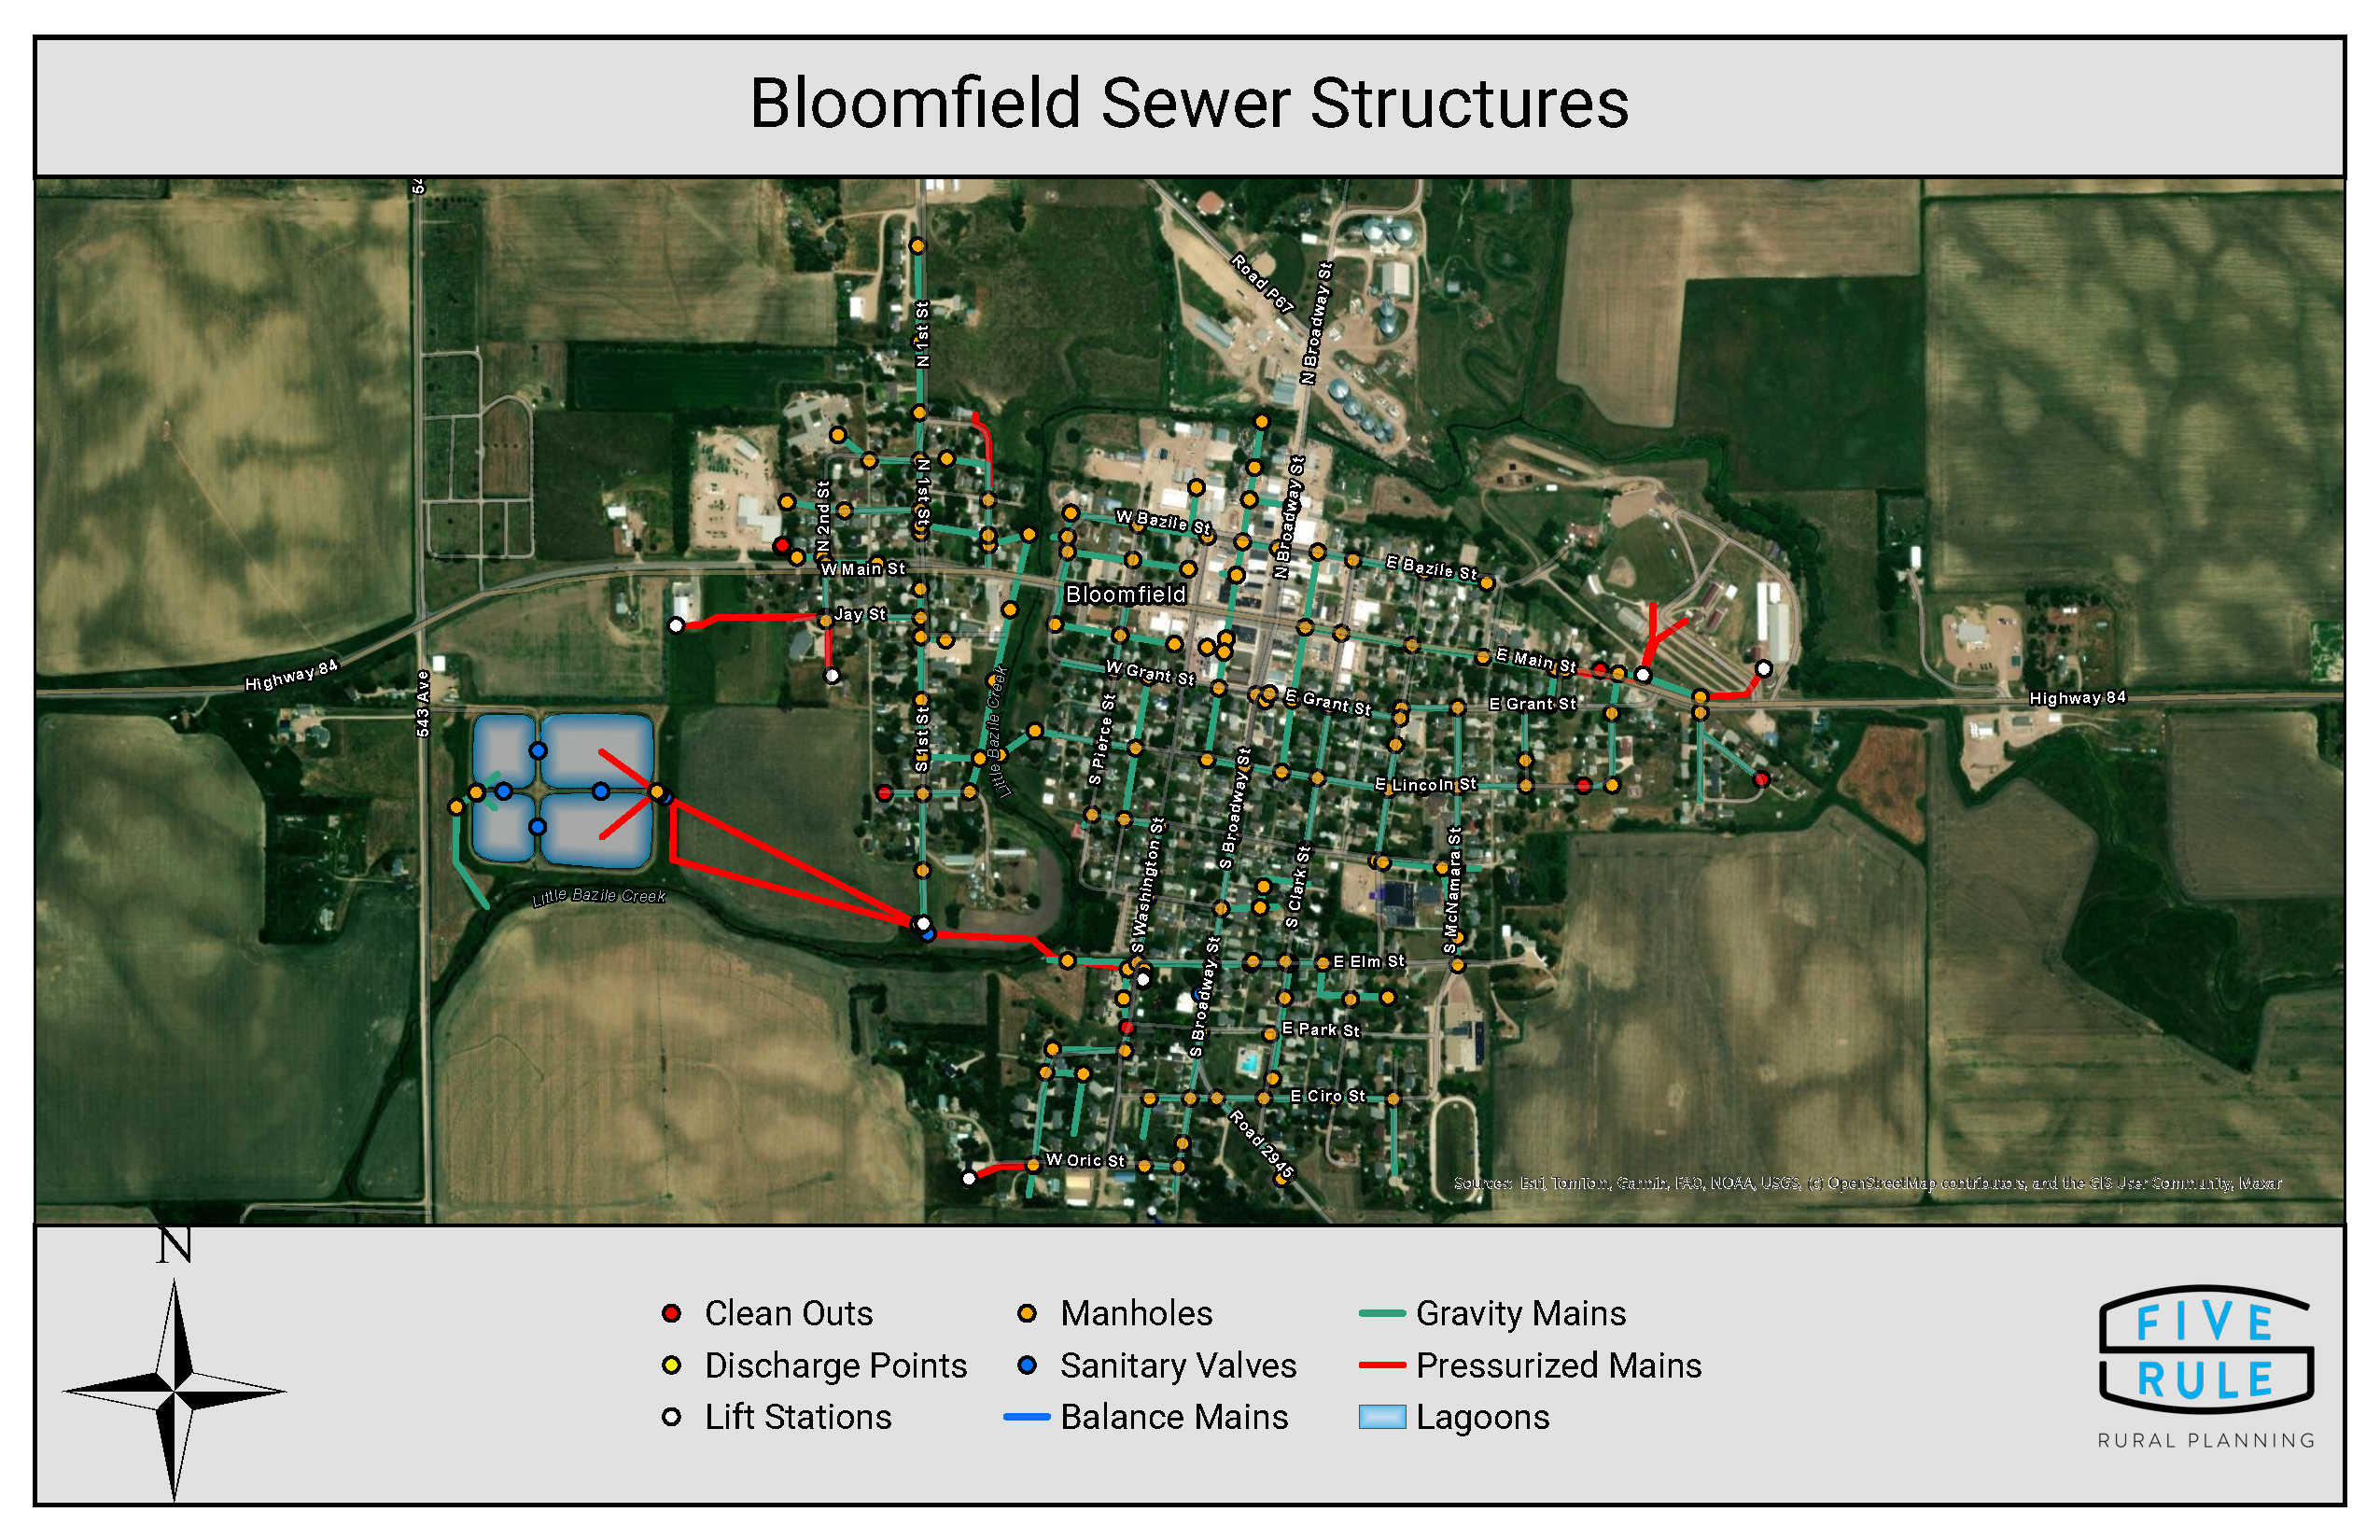
\includepdf[angle = 90]{maps/sewer_structures.pdf}
\end{landscape}

\pagebreak
\subsection{Energy Element}

\noindent As a reminder, \href{https://nebraskalegislature.gov/laws/statutes.php?statute=19-903}{NRS \S 19-903(4)} stipulates:

\begin{quote}
    (4) When a new comprehensive plan or a full update to an existing comprehensive plan is developed, an energy element which: Assesses energy infrastructure and energy use by sector, including residential, commercial, and industrial sectors; evaluates utilization of renewable energy sources; and promotes energy conservation measures that benefit the community.
\end{quote}

\noindent According to the \href{https://bloomfieldnebraska.com/government/}{Bloomfield City Government}, city residents have access to two sources of energy: electricity and natural gas. From the website:
\begin{quote}
"Electric service is supplied and distributed by the Nebraska Public Power District (NPPD). The nearest substation is located on the east edge of the community. The Bloomfield area is serviced by two different 69 KV lines. The transmission size to the substation is 69 KV and the substation capacity is 4160 KV with the distribution transformer approximately 60 percent loaded at the present. Two additional substations are located within five miles of Bloomfield. Service and maintenance is provided from the NPPD office in Norfolk."

Natural gas service is distributed and supplied to the community by SourceGas, through a three-inch transmission pipeline with an operating pressure of approximately 800-900 pounds per square inch. Choice Gas is available in Bloomfield and the election period for this program is prior to May 1st of each year.
\end{quote}

\noindent Most of Knox County's energy demand will be satisfied primarily by electricity and natural gas. Electricity consumption currently accounts for about two-thirds (68\%) of county consumption. By 2050, it is projected that share will increase to about three quarters (76\%). Furthermore, total costs are likely to increase for electricity but decrease or remain about the same for natural gas. As technology improves, electricity efficiency is likely to improve, driving per-unit costs down. On the other hand, natural gas efficiency is likely to get worse, driving per-unit costs up.

\begin{table}[H] 
\begin{framed}
\centering \doublespacing
  \caption{Knox County Energy Estimates}
  \label{table:energy}
 \scalebox{1.00}{
\begin{tabular}{l D{.}{.}{8.5} D{.}{.}{8.5} D{.}{.}{8.5}} \hline
\multicolumn{1}{c}{Year}& \multicolumn{1}{c}{Source} & \multicolumn{1}{c}{Consumption}  & \multicolumn{1}{c}{Cost}  \\ \hline
2020    & \multicolumn{1}{c}{Electricity}   & \multicolumn{1}{c}{197,390}   & \multicolumn{1}{c}{\$4,922,145}   \\
2020    & \multicolumn{1}{c}{Natural Gas}   & \multicolumn{1}{c}{93,489}    & \multicolumn{1}{c}{\$616,114}     \\
2030    & \multicolumn{1}{c}{Electricity}   & \multicolumn{1}{c}{208,019}   & \multicolumn{1}{c}{\$4,785,416}   \\
2030    & \multicolumn{1}{c}{Natural Gas}   & \multicolumn{1}{c}{85,745}    & \multicolumn{1}{c}{\$623,816}     \\
2040    & \multicolumn{1}{c}{Electricity}   & \multicolumn{1}{c}{227,321}   & \multicolumn{1}{c}{\$5,097,271}   \\
2040    & \multicolumn{1}{c}{Natural Gas}   & \multicolumn{1}{c}{80,929}    & \multicolumn{1}{c}{\$618,994}     \\
2050    & \multicolumn{1}{c}{Electricity}   & \multicolumn{1}{c}{252,633}   & \multicolumn{1}{c}{\$5,426,186}   \\
2050    & \multicolumn{1}{c}{Natural Gas}   & \multicolumn{1}{c}{78,031}    & \multicolumn{1}{c}{\$641,611}     \\
\hline
\end{tabular}
}
\floatnote{Data come from the \href{https://maps.nrel.gov/slope/data-viewer?filters=\%5B\%5D&layer=energy-consumption.net-electricity-and-natural-gas-consumption&year=2020\&res=county}{United States Department of Energy State and Local Planning for Energy database}. Consumption estimates are in Millions of British Thermal Units (MMBtu), while cost estimates are in nominal United States dollars.}
\end{framed}
\end{table}

\noindent In Nebraska, energy use is categorized according to land use. \textbf{Commercial energy} is used by non-manufacturing business establishments. This includes restauants, wholesale businesses, retail stores, and other service enterprises. Institutional and government offices and facilities are also included in the commercial sector, as well as streetlights, pumps, bridges, and other public services. \textbf{Residential energy} refers to energy used for private household functions, such as heating spaces, heating water, air conditioning, refrigeration, cooking, laundry, and lighting. \textbf{Figure~\ref{fig:energyElement}} displays projected energy consumptions and costs in Knox County between 2017 and 2050 across different land use categories.

\begin{figure}[H]
\centering
\begin{framed}
    \caption{Knox County Projected Energy Uses}
    \label{fig:energyElement}
     \begin{subfigure}{0.49\textwidth}
        \centering
        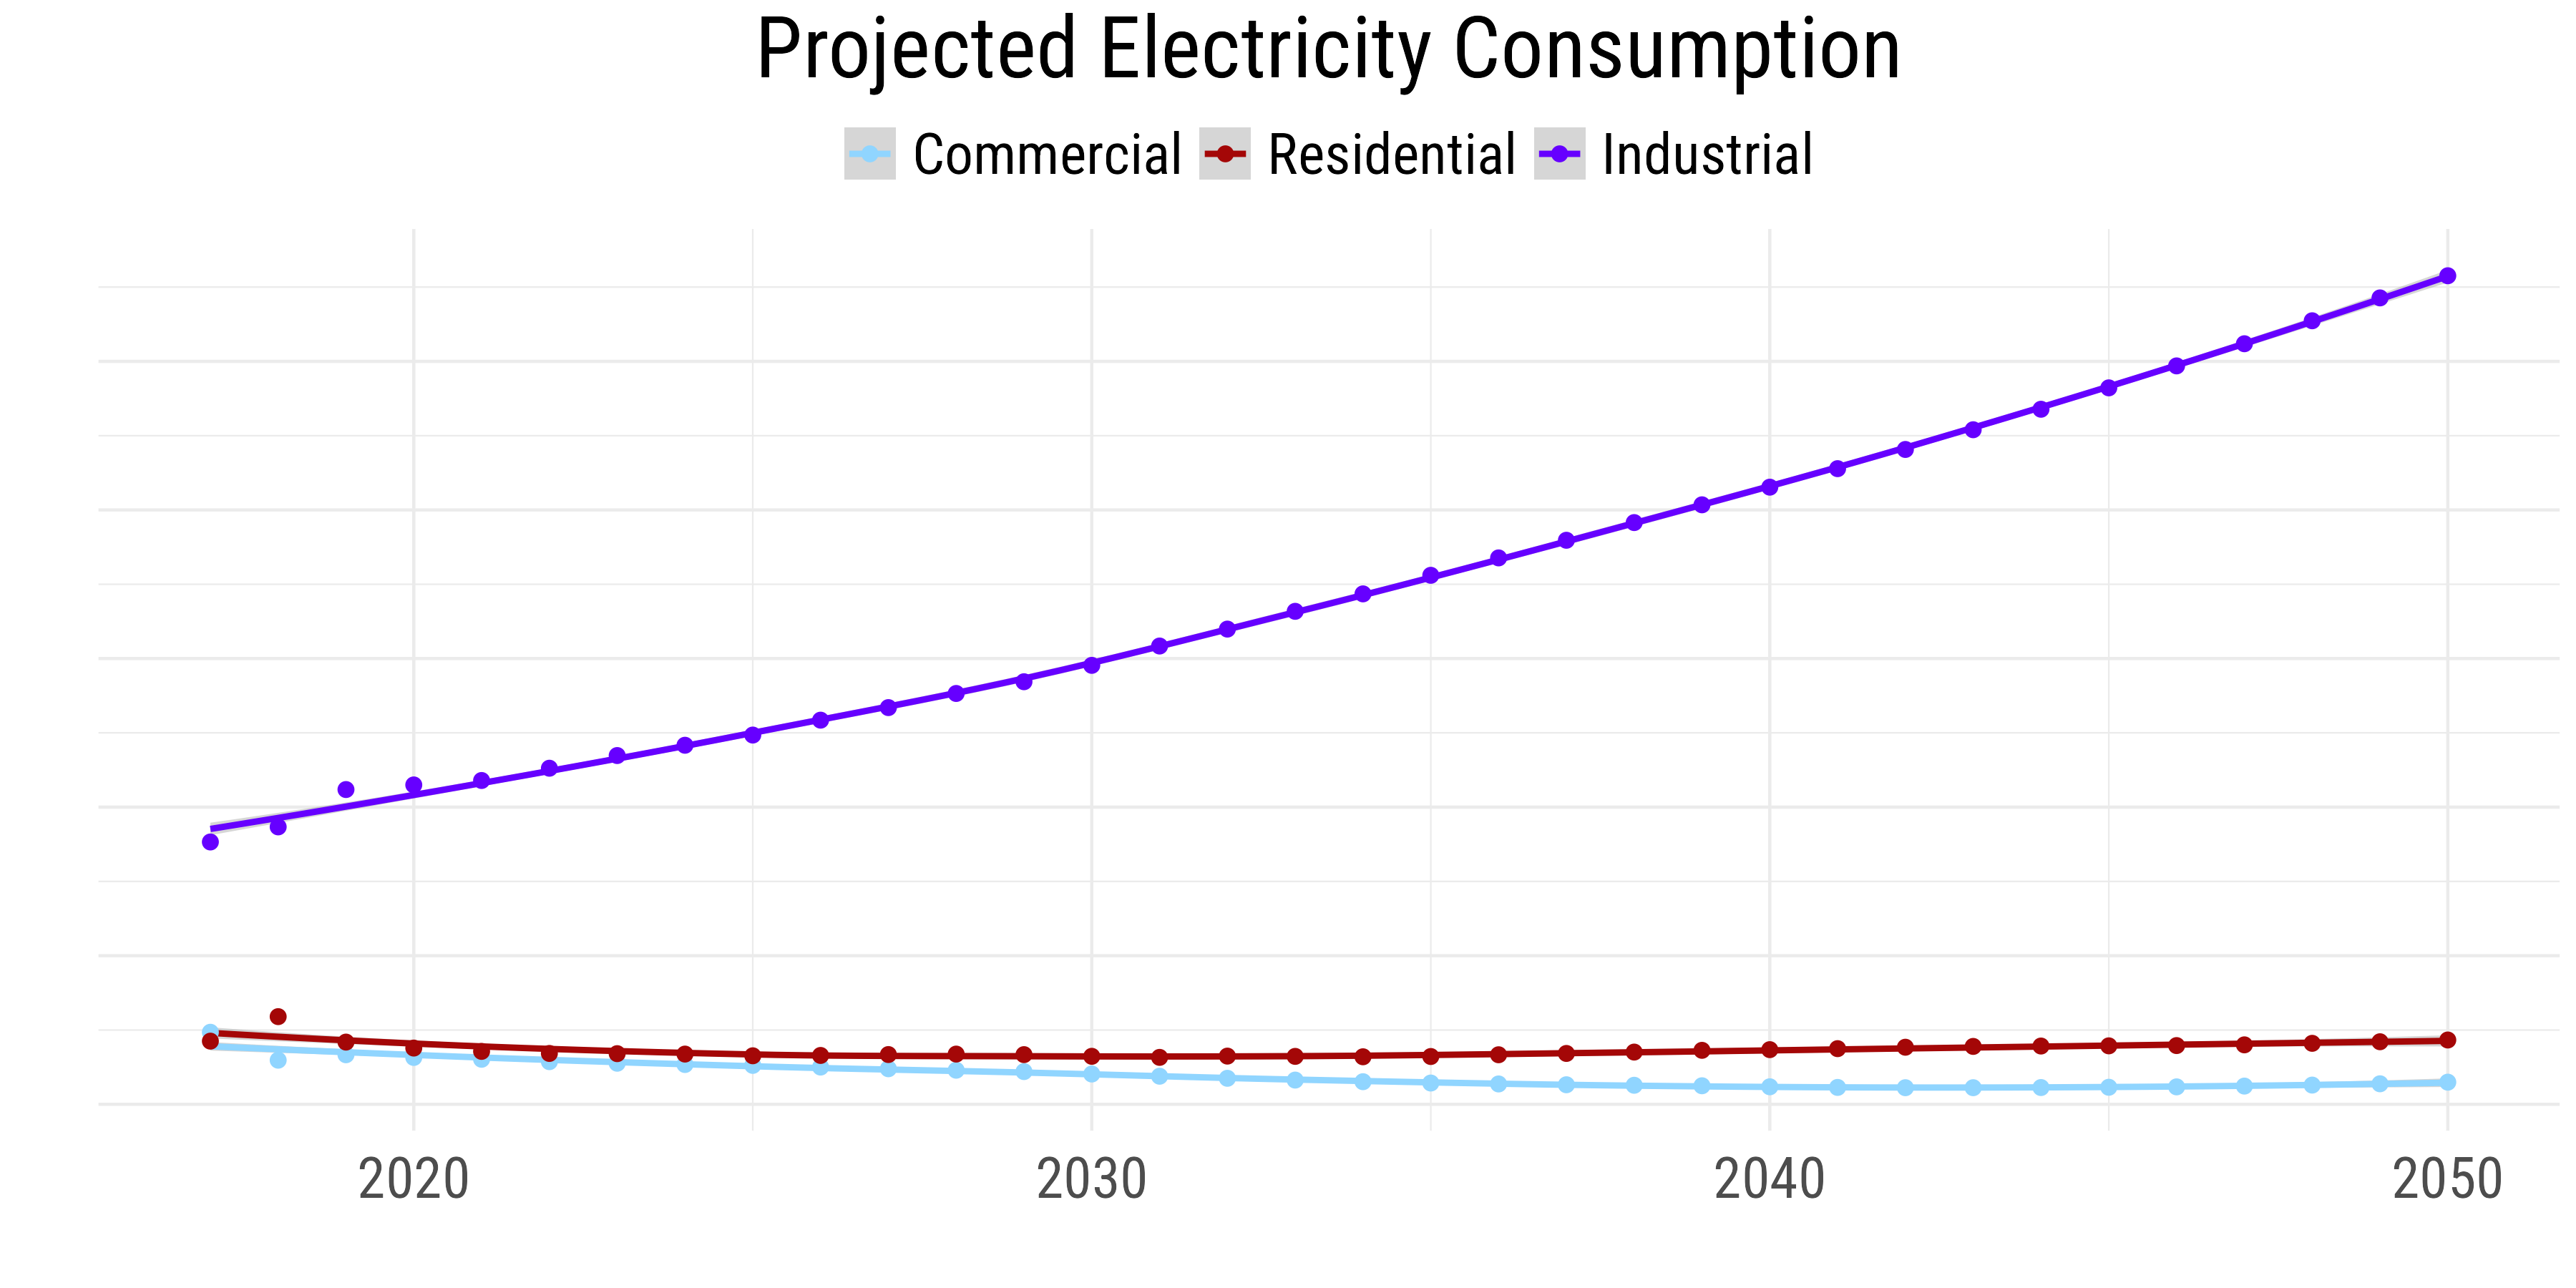
\includegraphics[width=\linewidth]{figures/energy_consumption_elec.png}
     \end{subfigure}
     \begin{subfigure}{0.49\textwidth}
        \centering
        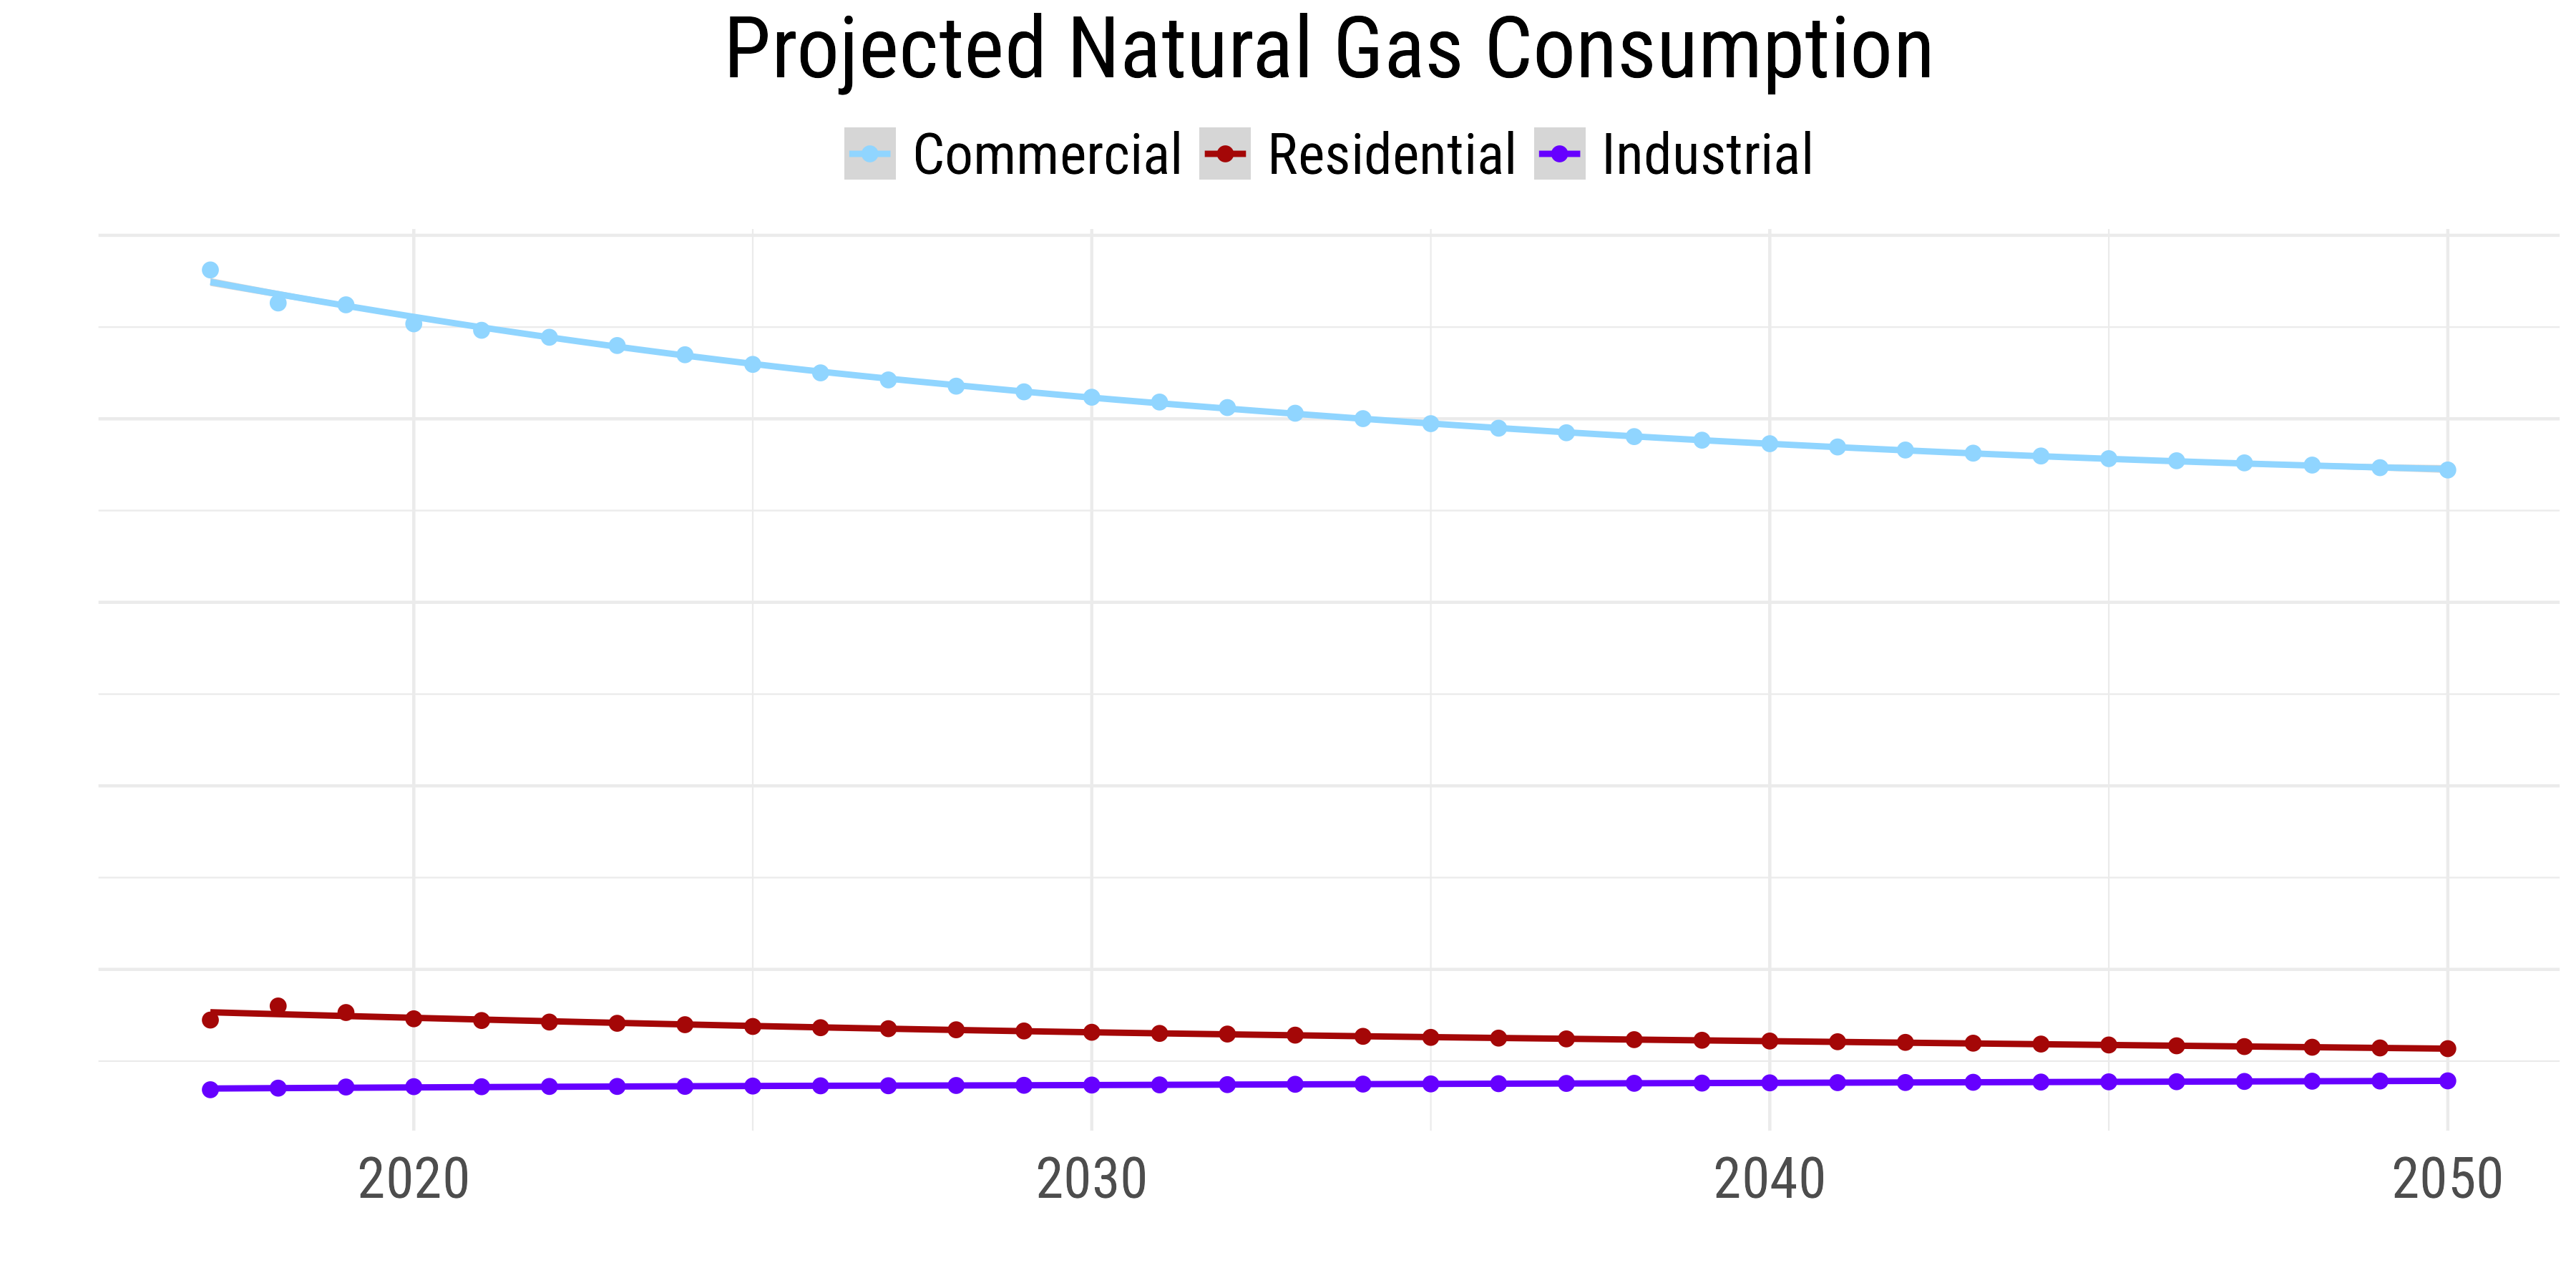
\includegraphics[width=\linewidth]{figures/energy_consumption_ng.png}
     \end{subfigure}
     \begin{subfigure}{0.49\textwidth}
        \centering
        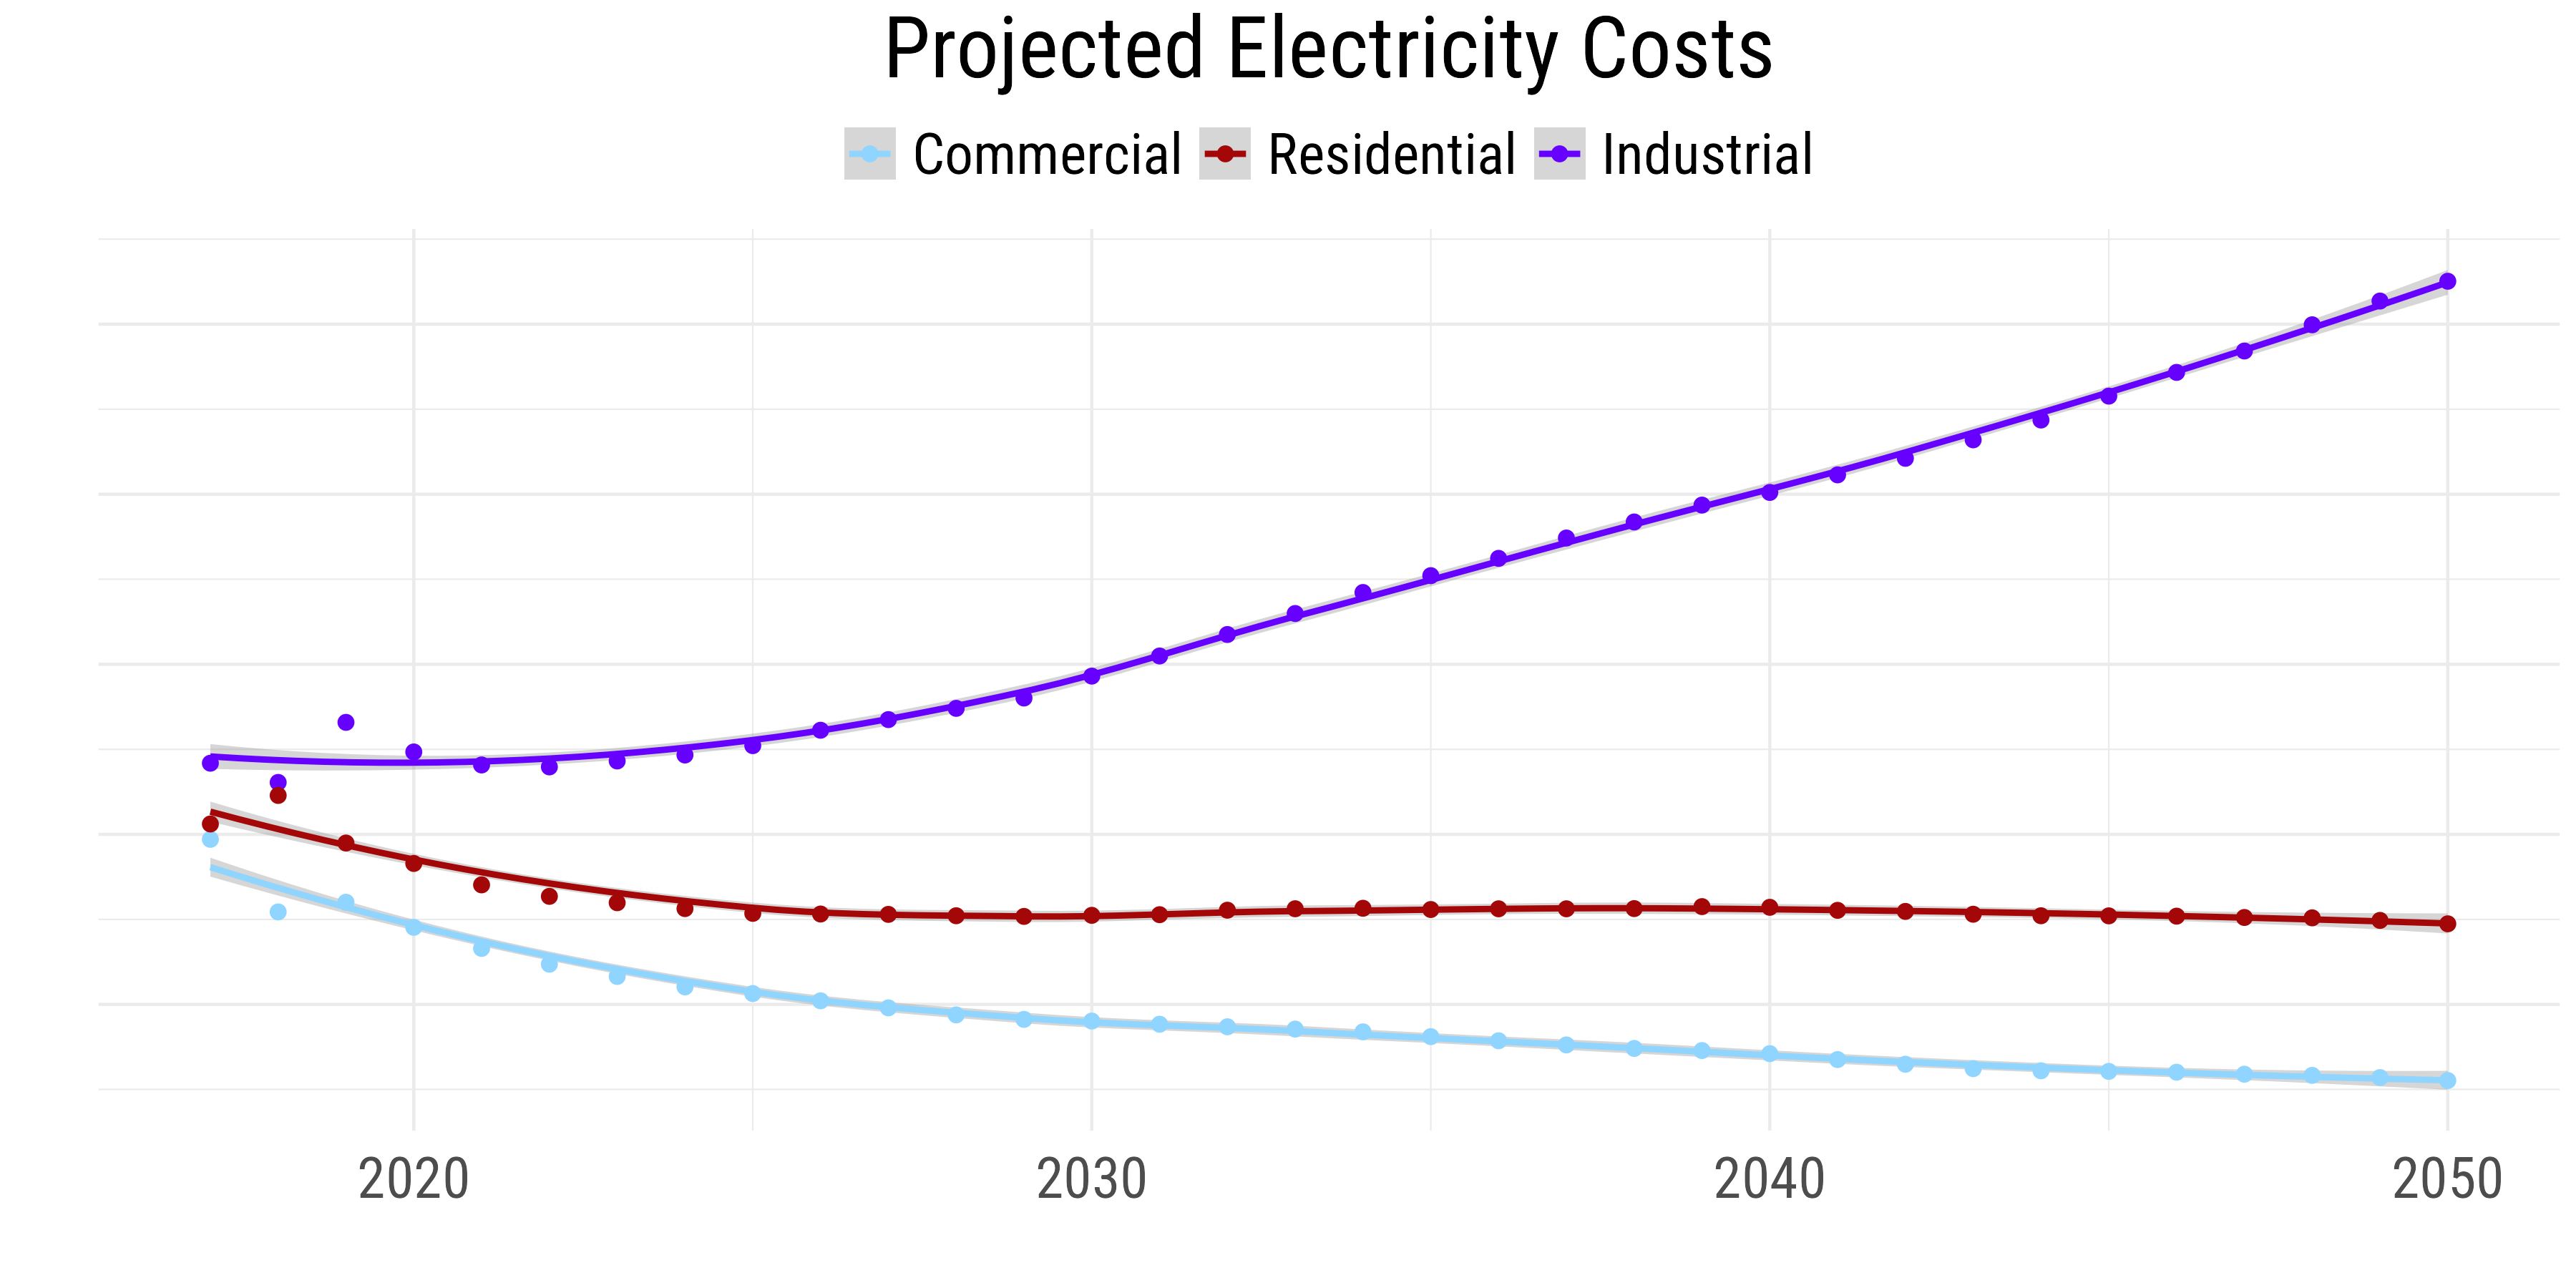
\includegraphics[width=\linewidth]{figures/energy_cost_elec.png}
     \end{subfigure}
     \begin{subfigure}{0.49\textwidth}
        \centering
        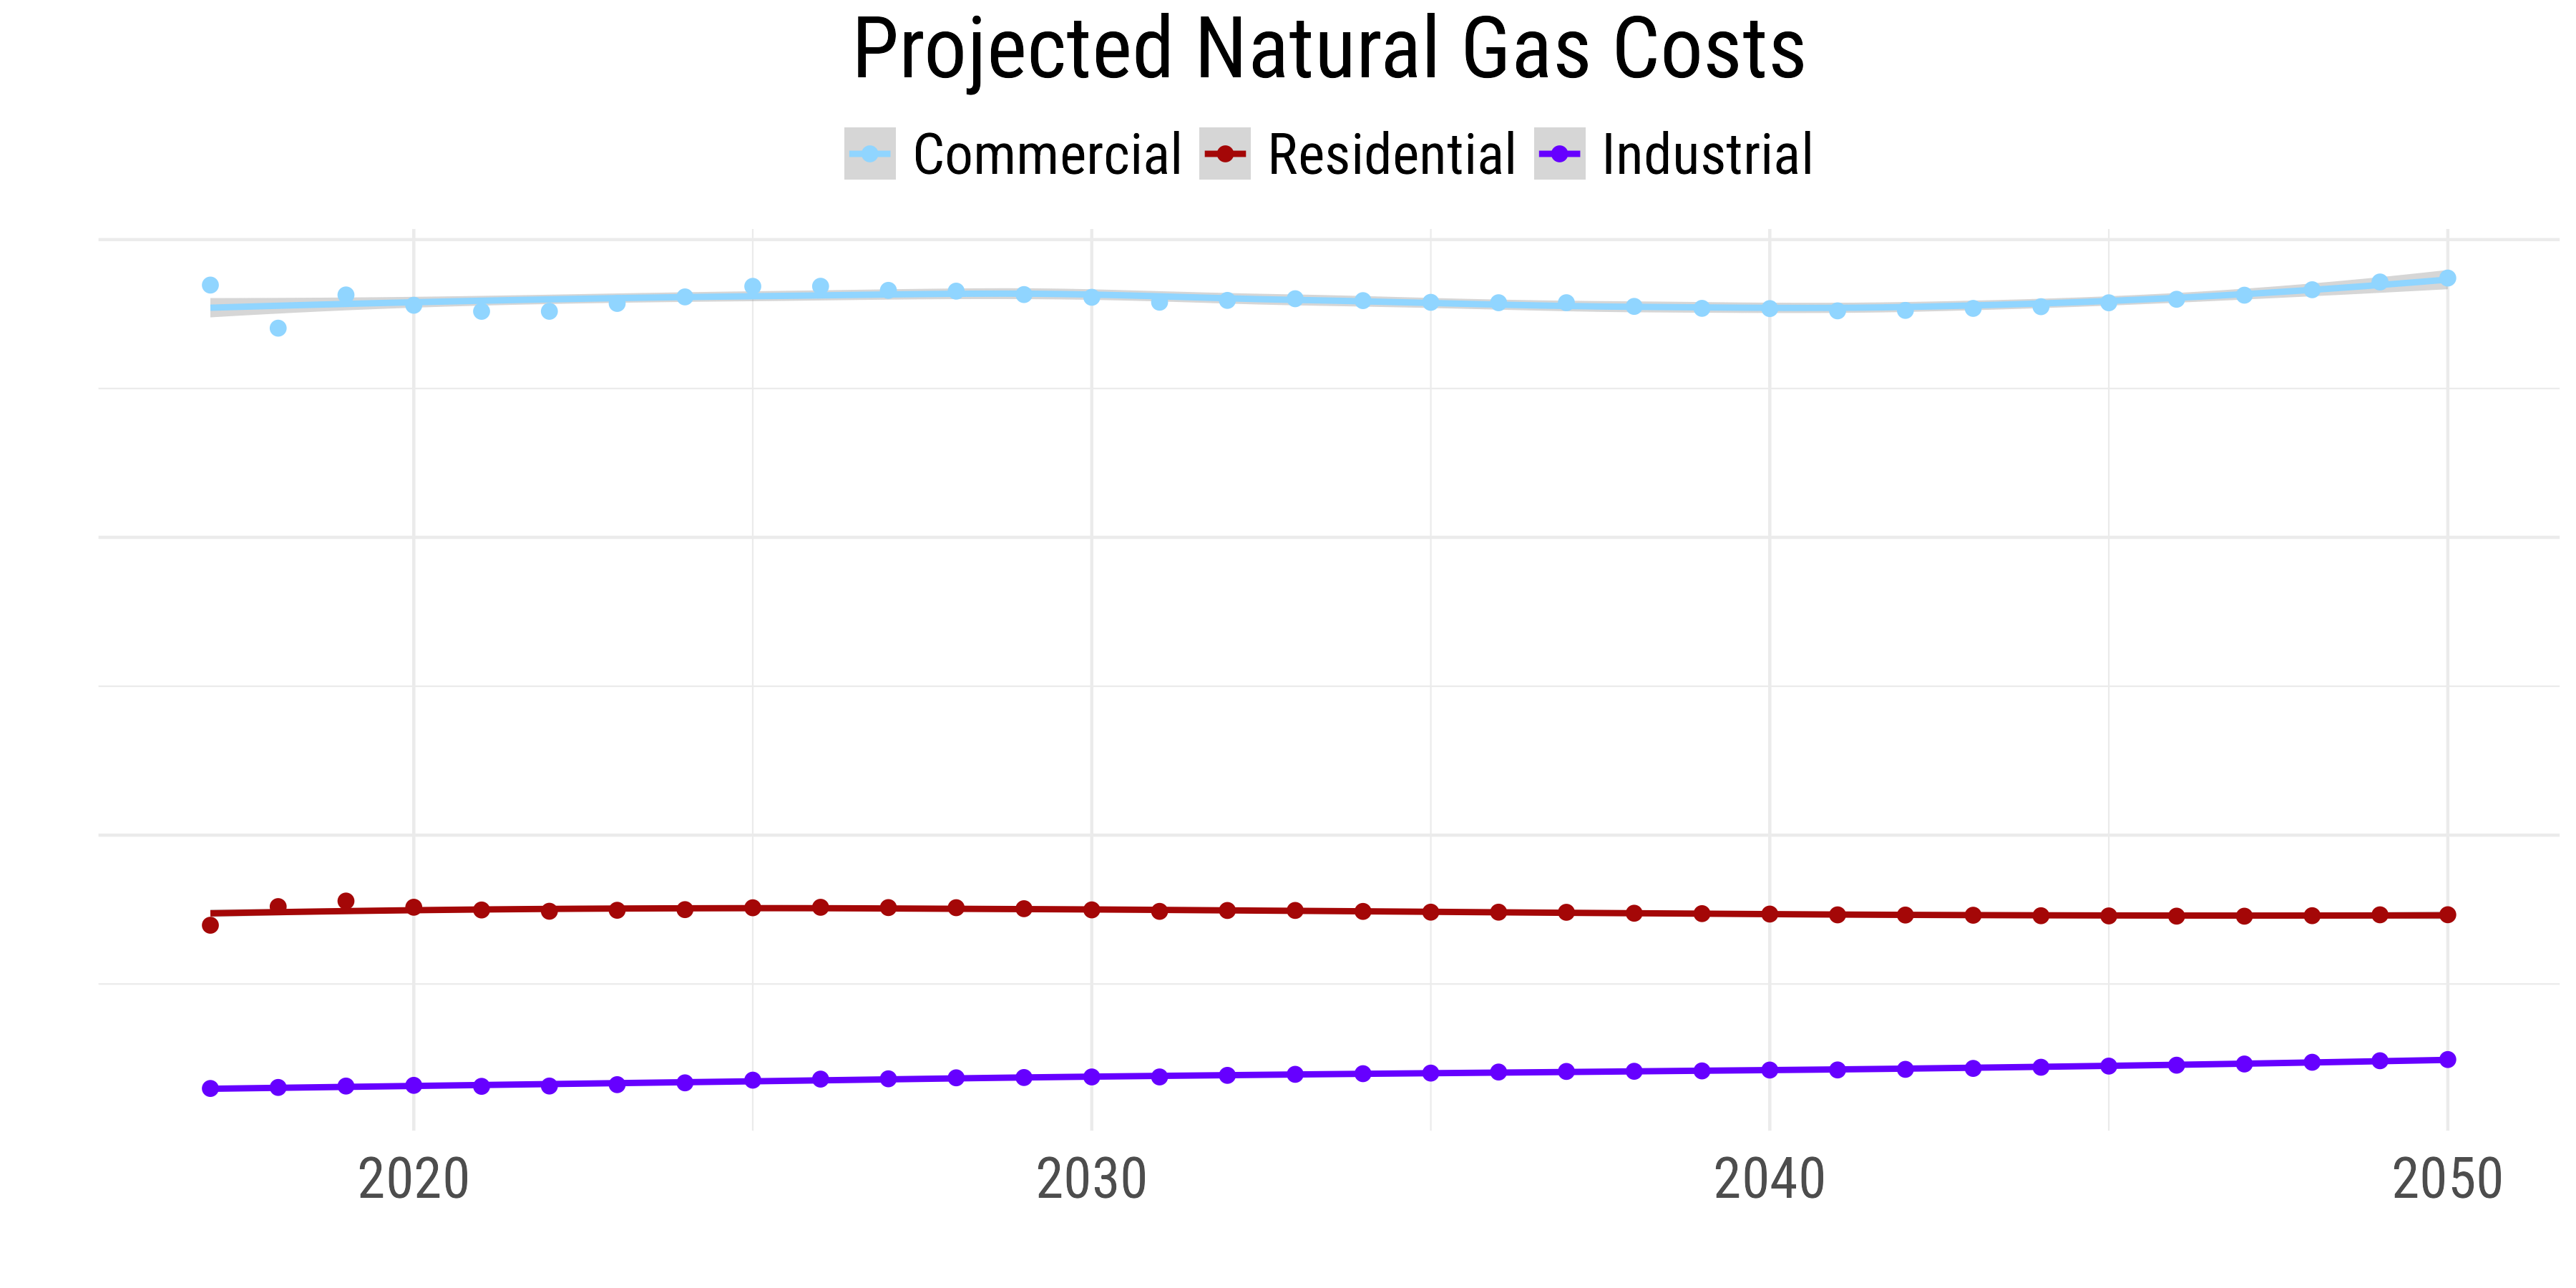
\includegraphics[width=\linewidth]{figures/energy_cost_ng.png}
     \end{subfigure}
    \rule[-5pt]{\linewidth}{0.4pt}
     \floatnote{Data come from the \href{https://maps.nrel.gov/slope/data-viewer?filters=\%5B\%5D&layer=energy-consumption.net-electricity-and-natural-gas-consumption&year=2020\&res=county}{United States Department of Energy State and Local Planning for Energy database}. All units are standardized to reflect relative, not absolute, growth and decline.}
\end{framed}
\end{figure}

\noindent Crucially, projected increase in electricity consumption and cost is likely to be driven entirely by industrial use, and to decrease in commercial and residential sectors. Overall decreases in commerical and residential energy consumption, across both sources, may be due to projected population decline across the county. If population trends reverse, expected consumption might also be projected to rise.

\subsubsection*{Renewable Resources}
\noindent \hl{[knox county has a windmill ban?]}

\pagebreak
\subsection{City Services}

\subsubsection*{Bloomfield Community Schools}

\noindent The \href{https://bloomfieldnebraska.com/education/}{City of Bloomfield Website} summarises the Bloomfield Community School District:

\begin{quote}
    Bloomfield Community School District 86R, is a Class 3 K-12 school district covering approximately 232 square miles. The elementary school and community auditorium/gymnasium were built in 1962. An addition to the elementary school was constructed in 1988 to accommodate special education, Chapter I programs and vocal music. The elementary school currently has a maximum capacity of 300. The elementary school building comprises 7,500-sq. ft. and has 19 classrooms. The auditorium/gymnasium building is 10,000-sq. ft. and also contains the vocational classrooms and shop areas. Vocational courses are currently offered at the high school level in the areas of industrial arts, agribusiness, home economics, and business. The high school also offers general education programs for adults, as well as a variety of special interest courses offered in cooperation with Northeast Community College in Norfolk and Wayne State College in Wayne. Graduate courses from Wayne State College and undergraduate courses from Northeast Community College are available.\\

    The Jr.-Sr. High School was built in 1927 and has been remodeled and updated several times. This building also has a maximum capacity of 300 and overall comprises 10,000-sq. ft. in the main building with 21 classrooms. A recent addition to the district was the installation of Distance Learning Technology over DS3 Fiber. The district has a student computer ratio of 1:4. Both the elementary and high school have a computer lab.
\end{quote}

\pagebreak
\subsubsection*{Public Lands, Buildings, and Services}

\noindent The City of Bloomfield owns multiple facilities that improve the quality of life for residents. The \href{https://bloomfieldnebraska.com/our-community/}{City of Bloomfield website} describes these facilities:

\subsubsection*{Ambulance Service}

\begin{quote}
    Established in 1969, the Bloomfield Ambulance Service is one of two ALS (Advanced Life Service) services in the county responding in the city of Bloomfield and the Bloomfield Fire District with the Bloomfield Fire Department. There are 18 state certified volunteer members of the department that include drivers, EMRs, EMTs, Paramedics and RNs with one full-time Paramedic. The department has monthly meetings/trainings and attend regularly scheduled county wide trainings. There is one ambulance in Bloomfield and one ambulance in Lindy, both of which are fully functional ALS ambulances carrying several medications, airway, trauma and 12 lead/defibrillation capable heart monitors.
\end{quote}

\subsubsection*{Fire Department}

\begin{quote}
    The City of Bloomfield Fire Department and Bloomfield Rural Fire Department operate as a volunteer organization with 35 members. The service area includes the City of Bloomfield and the surrounding rural fire district area consisting of approximately 342 square miles. On-going training and mutual aid coordination is handled at regular monthly meetings, with special training sessions provided several times each year. The fire trucks are in excellent condition and are well-equipped. The “jaws-of-life” is provided and operated by the Bloomfield Fire Department, which works in conjunction with the Bloomfield Ambulance Service. A thermal imaging camera, 1,800-gallon tanker, and a recent renovation to the fire hall enable the department to provide excellent service to the area.
\end{quote}

\subsubsection*{Police Department}

\begin{quote}
    The City of Bloomfield has a chief of police and one officer who have jurisdiction within the City and on all City property. The department provides full-time service. Communication and dispatching is through the Sheriff’s Office 911 system. The Knox County Sheriff’s Office, Nebraska State Patrol, Nebraska Game \& Parks, and Nebraska Fire Marshall also have jurisdiction.
\end{quote}

\subsubsection*{Community Center/City Hall}

\begin{quote}
    The Community Center and City Hall are located near the center of the business district. Built in 1995, this masonry structure is in excellent condition and is in compliance with ADA requirements. The building houses the city administrator’s office, clerk’s office, police department, and council chambers. The facility also offers a community room, which is utilized by various civic organizations including the senior citizens group for regular meetings and special events, such as potluck dinners. The city clerk’s office handles the reservations for the use of the community room.  The council room is also available for smaller groups. The American Legion Pavilion is also available for reservations. The American Legion Pavilion has air-conditioning and tables and chairs are included in reservation. The American Legion Pavilion now has an in-house speaker system for speaking and to play music through via Ipods and CDs.
\end{quote}

\subsubsection*{Library}

\begin{quote}
    The Bloomfield Public Library was organized in 1908. The Bloomfield Library Foundation completed a new public library building in 2000. The building houses the Bloomfield Public Library and Learning Center. High speed internet access is available on a number of public computers. The latest effort to boost technology includes participation in Library Broadband Builds Nebraska Communities, a project through the Nebraska Library Commission. Books, videos, cake pans, puzzles, puppets and cassette tapes are all available at the library.
\end{quote}

\pagebreak
\subsubsection*{Parks and Recreation}

\noindent The City of Bloomfield has two parks, a swimming pool, and the Knox County Fairgrounds. The \href{https://bloomfieldnebraska.com/our-recreation/}{City of Bloomfield website} describes several of them:

\subsubsection*{City Parks}
\begin{quote}
    The City of Bloomfield has two parks. The “City Park” is located in the south central part of the city. This park features a picnic shelter, horseshoe pits, two basketball hoops with concrete pads,  and restrooms.  The city park became home to new playground equipment in 2006. The second park is the “Robin Schulz Memorial Park.” This park is located in the north part of the city. The park features a lighted regulation size softball field with enclosed dugouts, sheltered bleachers, restrooms, equipment rooms, and a concession stand. A second softball field, added in 1997, features enclosed dugouts and a ground level pressbox.
\end{quote}

\subsubsection*{Swimming Pool}
\begin{quote}
    The municipal outdoor heated swimming pool was built in 1977, with a number of equipment replacements and upgrades since 1993, including the addition of a handicap accessibility lift system in 1994. The pool is located in the south central part of the city and is open from early June to early August. A picnic area with shelter is located adjacent to the swimming pool. A new slide and basketball hoop were added in 2000.
\end{quote}

\subsubsection*{Fairgrounds}
\begin{quote}
    The Knox County Fairgrounds, owned by the city, are located on the eastern edge of Bloomfield.  The fairgrounds contain a rodeo arena and livestock boarding, exhibition buildings, and camping spots with electrical outlets. In addition to the traditional buildings, the fairgrounds features a lighted baseball field with a concrete grandstand, restrooms, ticketbooth, and concession stand. Other features include a lighted football field.
\end{quote}

\pagebreak
\noindent Bloomfield residents have mixed evaluations of these facilities. \textbf{Figure~\ref{fig:scoreParks}} shows that they have positive evaluations of the fairgrounds and Robin Schulz Memorial Park, but neutral to negative evaluations of the Swimming Pool and City Park.

\begin{figure}[H]
\centering
\begin{framed}
    \caption{Community Assessment of Public Parks and Recreation}
    \label{fig:scoreParks}
    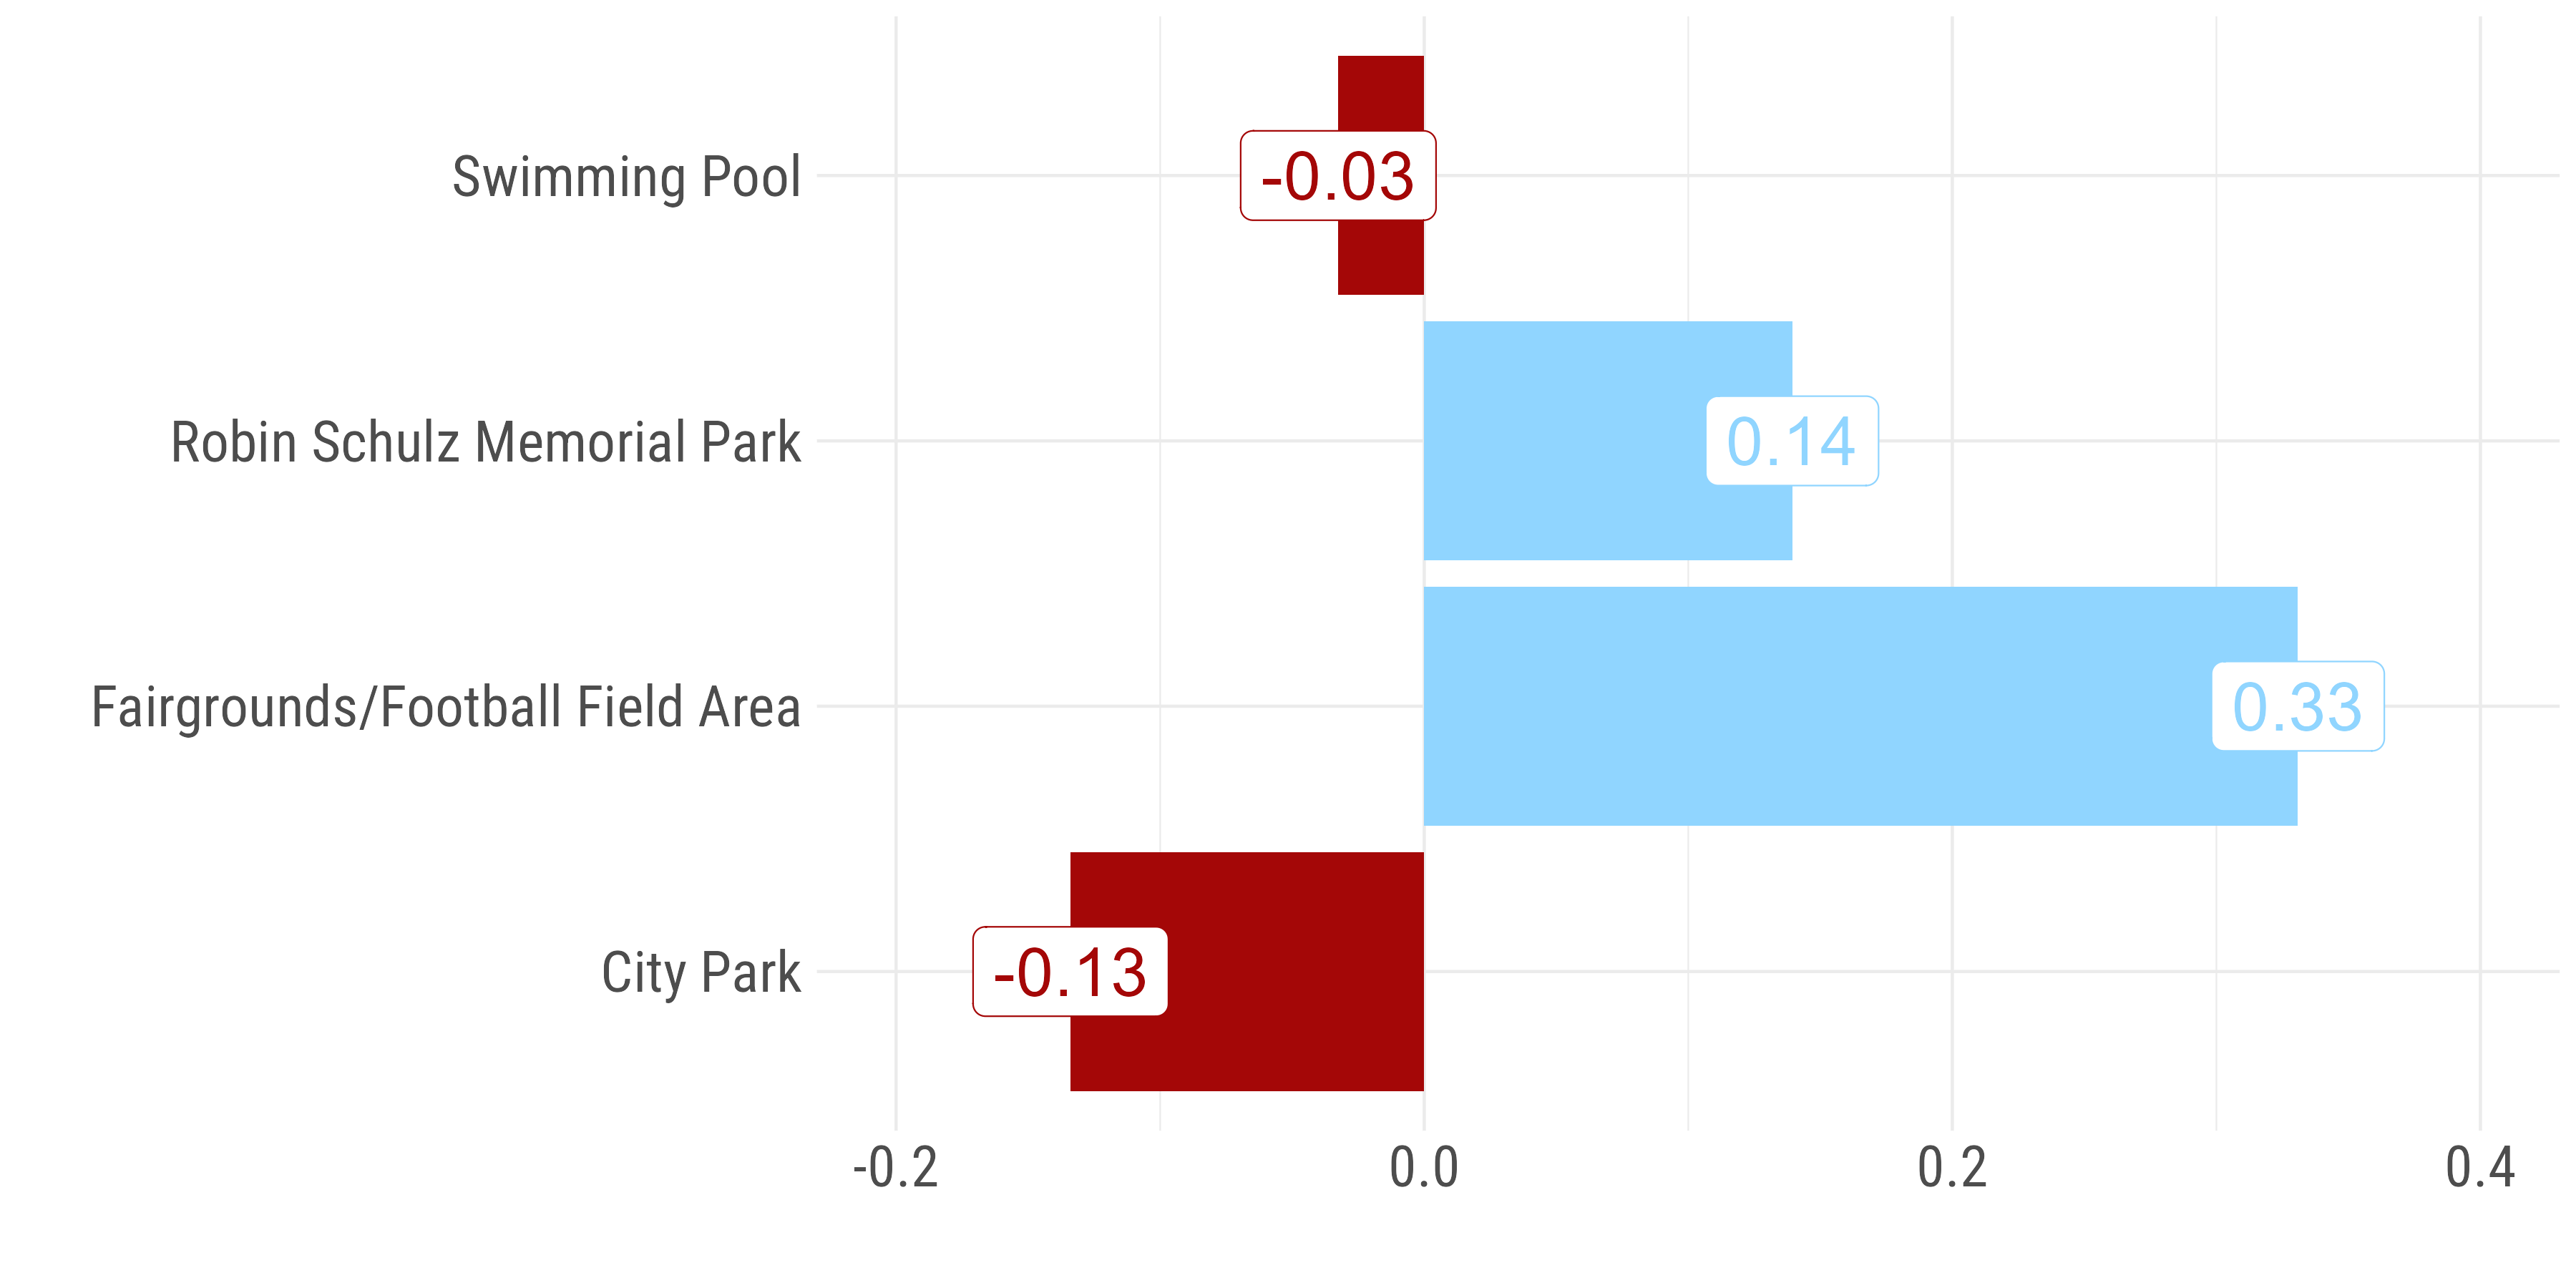
\includegraphics[width = \linewidth]{figures/score_parks.png}
\end{framed}
\end{figure}

\pagebreak
\subsubsection*{Bloomfield Municipal Airport}

\noindent \hl{[Is the airport owned by the city? I thought it was privately owned]}

\pagebreak
\subsection*{Key Takeaways}